% Компиляция: pdfLaTeX -> BibTeX -> pdfLaTeX -> pdfLaTeX
\documentclass[a4paper,12pt]{article}

\usepackage{cmap}
\usepackage[T2A]{fontenc}
\usepackage[utf8]{inputenc}
\usepackage[english,russian]{babel}
\usepackage{indentfirst}
\usepackage{amsmath,amssymb}
\usepackage{graphicx}
\usepackage[a4paper,top=2cm,bottom=2cm,left=2.5cm,right=2.5cm]{geometry}
\setlength{\emergencystretch}{1.5em}
\usepackage[numbers,sort&compress]{natbib}
\usepackage{booktabs}
\usepackage{tabularx}
\usepackage{array}
\usepackage[labelsep=period]{caption}
\usepackage{placeins}
\usepackage[hidelinks,pdfusetitle]{hyperref}

\renewcommand{\topfraction}{0.85}
\renewcommand{\bottomfraction}{0.6}
\renewcommand{\textfraction}{0.15}
\renewcommand{\floatpagefraction}{0.75}

\newcolumntype{L}{>{\raggedright\arraybackslash}X}
\newcolumntype{P}[1]{>{\raggedright\arraybackslash}p{#1}}

\title{Сходимость представлений нейросетей разных архитектур, модальностей
  и задач на примере рекомендательных систем}
% строку о научном руководителе можно добавить так:
% \\[2pt] \small Научный руководитель: И.\,О.~Фамилия
\author{В.\,А.~Талменев\\[2pt] \small Центральный университет, научный трек}
\date{}

\begin{document}

\maketitle

\begin{abstract}
Работа посвящена проверке гипотезы о~сходимости латентных представлений
глубоких нейронных сетей на рекомендательных системах. Согласно этой гипотезе,
модели разных архитектур, обученные на разных данных и~модальностях, с~ростом
масштаба приходят к~общей статистической модели реальности, однако для моделей,
обучаемых на истории взаимодействий пользователей с~товарами, она систематически
не проверялась. Цель работы~--- выяснить, сходятся ли векторные представления
товаров у~рекомендательных моделей разных архитектур между собой и~с~представлениями
описаний товаров в~больших языковых моделях, и~определить, какие факторы на это
влияют. Автором предлагается протокол сравнения представлений по совпадению
ближайших соседей и~по центрированному ядровому выравниванию с~поправкой
на случайный уровень, а~в~качестве эталона используется ядро поточечной взаимной
информации совместной встречаемости товаров. Протокол проверен на воспроизведении
исходного эксперимента: на 1024 парах «изображение~--- подпись» выравнивание пяти
языковых моделей BLOOMZ и~четырёх моделей зрения DINOv2 в~9--13 раз превышает
случайный уровень и~растёт с~размером обеих моделей. В~контролируемых экспериментах
на открытых наборах данных о~фильмах и~товарах для моделей матричного разложения,
последовательных трансформерных моделей и~языковых моделей разного размера
оценивается влияние размера модели, объёма данных, числа задач обучения
и~регуляризации на сходство представлений. Ожидается, что сходство окажется
частичным и~ограниченным общей информацией истории взаимодействий и~текстовых
описаний, а~сильные по качеству рекомендаций модели будут похожи друг на друга
сильнее, чем слабые. Полученные результаты позволят оценить применимость гипотезы
за пределами компьютерного зрения и~обработки текста и~использовать выравнивание
пространств для переноса знаний и~рекомендации новых товаров.

\medskip
\noindent\textit{Ключевые слова:} латентные представления, сходимость представлений,
платоновская гипотеза, рекомендательные системы, большие языковые модели,
сходство представлений.
\end{abstract}

%======================================================================
\section{Введение}

Современные модели машинного обучения становятся всё более универсальными:
одни и~те же архитектуры и~предобученные модели применяются к~текстам, изображениям
и~другим видам данных. Отталкиваясь от этого наблюдения, Huh и~соавторы~\cite{huh2024platonic}
выдвинули платоновскую гипотезу представлений, согласно которой нейронные сети,
обученные на разных данных, задачах и~модальностях, с~ростом масштаба сходятся
к~общей статистической модели реальности. Под латентным представлением здесь
понимается вектор, в~который модель переводит объект, а~под сходимостью~--- рост
совпадения структуры сходства объектов в~пространствах разных моделей. Гипотеза
проверялась в~основном на моделях компьютерного зрения и~обработки естественного
языка~\cite{huh2024platonic,maniparambil2024,sharma2024checkup}. Рекомендательные
системы относятся к~наиболее массовым приложениям машинного обучения~\cite{zhai2024hstu},
но представления товаров в~них строятся по истории взаимодействий пользователей,
а~не по текстам или изображениям~\cite{kang2018sasrec,sun2019bert4rec}.
Распространяется ли на такие модели сходимость представлений, неизвестно, хотя
от ответа на этот вопрос зависят перенос знаний между моделями, рекомендация новых
товаров и~выбор моделей без размеченных данных.

Основания для гипотезы дают работы о~совместимости представлений. Слои разных сетей
удаётся соединять между собой без потери качества~\cite{lenc2015equivariance,bansal2021stitching},
представления разных моделей~--- сравнивать через сходство с~общими опорными
объектами~\cite{moschella2023relative}, а~в~независимо обученных моделях находятся
общие нейроны~\cite{dravid2023rosetta}. Совместимость сохраняется и~между модальностями:
представления моделей зрения переводятся в~пространство языковой модели линейным
отображением~\cite{merullo2023linearly}, а~выравнивание моделей зрения и~языка растёт
вместе с~их качеством~\cite{huh2024platonic,maniparambil2024}. Сильная версия гипотезы
позволяет переводить векторные представления текстов из пространства одной модели
в~пространство другой вообще без парных данных~\cite{jha2025vec2vec}, а~для
совместно-встраивающих предсказательных архитектур (JEPA) сходимость доказана
теоретически~\cite{balestriero2026jepa}. В~рекомендательных системах модели,
построенные на текстовых описаниях товаров, конкурируют с~моделями
на идентификаторах~\cite{hou2022unisrec,li2023recformer,yuan2023idvsmodality}.
Наиболее близкий к~настоящей работе результат получен в~\cite{sheng2025alpharec}:
представления названий товаров из языковых моделей после линейного отображения
обеспечивают коллаборативную фильтрацию лучше, чем модели на идентификаторах.
Это указывает на родство языкового пространства и~пространства поведения
пользователей.

Вместе с~тем экспериментальная база гипотезы уязвима. Выравнивание
в~\cite{huh2024platonic} измерено на 1024 парах «изображение~--- подпись»
с~однозначным соответствием; при увеличении выборки тренд почти исчезает,
а~в~режиме «многие ко многим» выравнивание резко снижается~\cite{koepke2026cave}.
Распространённые меры сходства завышаются с~ростом глубины и~ширины модели: после
калибровки глобальная сходимость почти пропадает и~сохраняется лишь согласие
локальных окрестностей~\cite{groger2026aristotelian}. Кроме того, значение
центрированного ядрового выравнивания (CKA) можно существенно изменить, не меняя
поведения модели~\cite{davari2023cka}. Работы о~рекомендательных
системах~\cite{hou2022unisrec,li2023recformer,yuan2023idvsmodality,sheng2025alpharec}
оценивают качество рекомендаций, но не сходство геометрии пространств и~его
зависимость от масштаба. Модели на идентификаторах и~на текстах дополняют друг
друга~\cite{collins2025complementarity}, что говорит скорее о~частичной, чем о~полной
сходимости. Сходство представлений рекомендательных моделей измерялось лишь
в~отдельных работах и~без связи с~гипотезой~\cite{iana2024peeling},
а~в~\cite{lin2024dreamumm} гипотеза используется как основа метода рекомендаций,
но сама не проверяется. Систематической проверки сходимости представлений для
рекомендательных моделей пока нет.

В~настоящей работе предлагается провести такую проверку. Её цель~--- выяснить,
сходятся ли векторные представления товаров у~рекомендательных моделей разных
архитектур между собой и~с~представлениями описаний товаров в~больших языковых
моделях, и~определить, какие факторы на это влияют. Для этого представления товаров
сравниваются у~моделей разных архитектур~--- матричного разложения,
Item2Vec~\cite{barkan2016item2vec}, SASRec~\cite{kang2018sasrec}
и~BERT4Rec~\cite{sun2019bert4rec}~--- между собой, а~также с~представлениями описаний
тех же товаров в~языковых моделях разного размера. Сходство измеряется по совпадению
ближайших соседей~\cite{huh2024platonic} и~по CKA~\cite{kornblith2019cka} с~калибровкой
относительно случайного уровня~\cite{groger2026aristotelian}. Эталоном служит ядро
поточечной взаимной информации совместной встречаемости товаров: согласно теоретическим
результатам~\cite{huh2024platonic,oord2018cpc,levy2014implicit}, именно к~нему сходятся
модели, обученные на совместной встречаемости. Влияние факторов, на которые указывает
гипотеза~\cite{huh2024platonic},~--- размера модели, объёма данных, числа задач
и~регуляризации~--- оценивается в~контролируемых экспериментах. В~отличие
от~\cite{sheng2025alpharec}, в~работе изучается не качество рекомендаций, а~геометрия
пространств представлений, а~в~отличие от~\cite{huh2024platonic} учитывается критика
мер сходства~\cite{koepke2026cave,groger2026aristotelian}.

Для достижения поставленной цели работа выполняется в~несколько этапов. Сначала
проводится обзор литературы и~воспроизводится эксперимент~\cite{huh2024platonic}
по выравниванию моделей зрения и~языка на открытых данных с~использованием кода
авторов. Далее строится протокол сравнения представлений товаров, включающий локальные
и~глобальные меры сходства, их калибровку, базовую линию из моделей одной архитектуры
с~разной инициализацией и~эталон по совместной встречаемости. Затем обучается набор
рекомендательных моделей разных архитектур и~размеров, измеряется сходство
их представлений между собой и~с~языковыми моделями и~оценивается влияние размера
модели, объёма данных, многозадачности и~регуляризации. Завершает работу проверка
практических следствий: рекомендации новых товаров в~условиях холодного старта через
линейный перевод из языкового пространства и~связи выравнивания с~качеством
рекомендаций.

Эксперименты планируется провести на открытых наборах данных MovieLens и~Amazon
Reviews, которые содержат как истории взаимодействий пользователей, так и~текстовые
описания товаров. Представления описаний строятся языковыми моделями нескольких
размеров. Сходство представлений оценивается по совпадению взаимных $k$ ближайших
соседей (mutual $k$-NN) при нескольких значениях~$k$, по CKA и~по его локальному
варианту CKNNA~\cite{huh2024platonic} с~калибровкой~\cite{groger2026aristotelian},
а~качество рекомендаций~--- метриками Recall@$K$ и~NDCG@$K$.

Основной результат работы~--- протокол проверки сходимости представлений для
рекомендательных моделей, дающий количественную оценку степени и~факторов сходимости
и~отличающийся калибровкой мер сходства и~эталоном на основе совместной встречаемости
товаров. С~его помощью предполагается оценить степень сходимости рекомендательных
и~языковых моделей и~её предел, заданный общей информацией истории взаимодействий
и~текстовых описаний, а~также влияние размера модели, объёма данных, многозадачности
и~регуляризации. Практическое значение работы связано с~рекомендацией новых товаров
через линейный перевод из языкового пространства и~с~выбором модели по степени
выравнивания. Обзор работ, на которых основана постановка задачи, приведён
в~разделе~\ref{sec:review}, сама постановка~--- в~разделе~\ref{sec:problem}.
В~разделе~\ref{sec:exp0} описано воспроизведение эксперимента~\cite{huh2024platonic},
в~разделе~\ref{sec:plan}~--- план экспериментов с~рекомендательными моделями.

%======================================================================
\section{Обзор литературы}\label{sec:review}

Работы, относящиеся к~теме, можно разделить на четыре группы: эмпирические
свидетельства сходимости представлений, меры сходства и~их критика, теоретические
объяснения сходимости и~исследования представлений в~рекомендательных системах.
Первые три группы отвечают на вопрос, сходятся ли представления и~как это измерить,
четвёртая показывает, что известно о~представлениях товаров.

Ранние свидетельства сходимости получены методом склейки~\cite{lenc2015equivariance,bansal2021stitching}:
слои одной сети соединяются со слоями другой через обучаемый линейный слой, и~качество
решения задачи при этом сохраняется. Ранние слои оказываются взаимозаменяемыми лучше
глубоких, а~сети, обученные на разные задачи, совместимы лишь
частично~\cite{lenc2015equivariance}. Относительные представления~\cite{moschella2023relative}
и~общие нейроны в~наборе разнородных моделей~\cite{dravid2023rosetta} демонстрируют
совместимость без обучения стыковки, а~сходство весов с~точностью до перестановки
нейронов позволяет объединять независимо обученные модели~\cite{ainsworth2023rebasin}.
Совместимость обнаруживается и~между модальностями. Модели зрения связываются
с~языковыми линейной проекцией~\cite{merullo2023linearly}; сильные модели
представления изображений, обученные как с~текстовыми подписями~\cite{radford2021clip},
так и~без них~\cite{oquab2024dinov2}, семантически близки к~языковым~\cite{maniparambil2024},
а~языковые модели, не видевшие изображений, отражают визуальную структуру
мира~\cite{sharma2024checkup,abdou2021color}. В~\cite{huh2024platonic} эти наблюдения
обобщены в~гипотезу о~том, что выравнивание моделей растёт с~их качеством и~масштабом,
а~в~\cite{jha2025vec2vec} её сильная версия подтверждена переводом векторных
представлений текстов между моделями без парных данных. Нерешённым, однако, остаётся
вопрос, выполняется ли гипотеза за пределами зрения и~текста.

Выводы о~сходимости напрямую зависят от того, как измеряется сходство представлений.
Долгое время стандартом служило CKA~\cite{kornblith2019cka}; обзоры~\cite{klabunde2025survey,sucholutsky2023aligned}
систематизируют десятки мер и~отмечают, что они нередко дают разные ответы. Недостаток
CKA~--- чувствительность к~удалённым точкам: его значение можно сильно изменить,
не изменив поведения модели~\cite{davari2023cka}. В~\cite{huh2024platonic} вместо него
используется локальная мера~--- совпадение $k$ ближайших соседей (mutual $k$-NN)~---
и~промежуточная между ними мера CKNNA. Работы 2026~года показывают, что и~эти оценки
ненадёжны. При росте выборки с~1024 пар до миллионов тренд выравнивания почти исчезает,
число соседей~$k$ приходится увеличивать вместе с~выборкой, а~в~режиме «многие ко многим»
выравнивание падает~\cite{koepke2026cave}. Меры сходства систематически завышаются
с~ростом глубины и~ширины сети; после перестановочной калибровки глобальная сходимость
исчезает, а~согласие локальных окрестностей сохраняется~\cite{groger2026aristotelian}.
Следовательно, вывод о~сходимости зависит от выбранной меры и~режима оценки, поэтому
измерять её нужно несколькими мерами с~калибровкой.

Теоретические работы объясняют, к~чему должны сходиться представления.
В~\cite{huh2024platonic} показано, что в~идеализированном мире, где наблюдения
не теряют информации, контрастные модели любой модальности сходятся к~одному ядру~---
поточечной взаимной информации событий. Этот результат опирается на свойства
контрастной функции потерь~\cite{oord2018cpc} и~согласуется с~тем, что word2vec неявно
раскладывает матрицу такой информации~\cite{levy2014implicit}. В~\cite{balestriero2026jepa}
доказано, что совместно-встраивающие предсказательные архитектуры, обученные на разных
модальностях, приходят к~одному представлению с~точностью до поворота, если положительные
пары образованы двумя видами одной сцены. Слабое место обоих объяснений~---
идеализированные допущения: в~реальных данных наблюдения теряют информацию, и~сходимость
ограничена общей для модальностей частью~\cite{huh2024platonic}. Для рекомендательных
систем эта теория важна непосредственно, поскольку многие из них являются моделями
совместной встречаемости товаров~\cite{barkan2016item2vec}, и~эталонное ядро можно
вычислить прямо по данным.

Представления товаров в~рекомендательных системах изучаются в~основном с~точки зрения
качества рекомендаций. Классические последовательные модели строят их по идентификаторам
товаров~\cite{kang2018sasrec,sun2019bert4rec}, иногда с~дополнительной контрастной
задачей~\cite{xie2022cl4srec}, а~крупные генеративные модели этого класса подчиняются
законам масштабирования~\cite{zhai2024hstu}. Работы~\cite{hou2022unisrec,li2023recformer,yuan2023idvsmodality}
заменяют идентификаторы представлениями текстов и~изображений и~показывают, что такие
модели сравнимы с~моделями на идентификаторах и~лучше переносятся между доменами.
В~\cite{sheng2025alpharec} линейное отображение представлений названий товаров
из языковой модели в~пространство поведения превосходит ведущие модели
на идентификаторах; авторы объясняют это гомоморфизмом языкового и~поведенческого
пространств. Рекомендательные системы на основе больших языковых моделей действуют
в~обратном направлении: они переводят коллаборативные представления в~пространство
языковой модели небольшим проектором~\cite{zhang2023collm,liao2024llara} или строят
семантические идентификаторы из представлений содержимого~\cite{rajput2023tiger}.
Сходство представлений как таковое исследуется лишь в~отдельных работах.
В~\cite{collins2025complementarity} показано, что модели на идентификаторах и~на тексте
дополняют друг друга, а~в~\cite{iana2024peeling} представления новостных рекомендательных
моделей с~разными кодировщиками сравниваются мерой CKA и~по пересечению списков
рекомендаций, и~делается вывод, что по одному лишь качеству рекомендаций нельзя судить
о~сходстве моделей. Работа~\cite{lin2024dreamumm} строит метод рекомендаций на основе
гипотезы~\cite{huh2024platonic}, но не проверяет её.

Сильные и~слабые стороны рассмотренных подходов сопоставлены в~табл.~\ref{tab:review}.
Общий недостаток работ о~сходимости состоит в~том, что их выводы получены для зрения
и~языка и~чувствительны к~выбору меры, тогда как работы о~рекомендательных системах
оценивают пользу языковых представлений, не измеряя саму сходимость.

\begin{table}[!htbp]
\caption{Сравнение подходов к~изучению сходства представлений}
\label{tab:review}
\small
\renewcommand{\arraystretch}{1.15}
\begin{tabularx}{\textwidth}{@{}P{3.7cm}P{1.6cm}LL@{}}
\toprule
Подход & Работы & Достоинства & Недостатки \\
\midrule
Склейка и~относительные представления
  & \cite{moschella2023relative,bansal2021stitching,dravid2023rosetta,lenc2015equivariance}
  & Прямо проверяют совместимость представлений
  & Требуется обученная стыковка или набор опорных объектов; нет единой меры сходимости \\
\addlinespace[2pt]
Выравнивание по ближайшим соседям между модальностями
  & \cite{huh2024platonic,maniparambil2024,sharma2024checkup,merullo2023linearly}
  & Простая мера; виден рост сходства с~масштабом
  & Оценка на 1024 парах «один к~одному»; чувствительность к~$k$ и~размеру
    выборки~\cite{koepke2026cave} \\
\addlinespace[2pt]
Глобальные меры и~калибровка
  & \cite{groger2026aristotelian,kornblith2019cka,klabunde2025survey,davari2023cka}
  & Хорошо изучены; калибровка устраняет смещение от размера
    модели~\cite{groger2026aristotelian}
  & Значение CKA легко изменить, не меняя поведения модели~\cite{davari2023cka};
    без калибровки сходство завышается \\
\addlinespace[2pt]
Перевод между пространствами без парных данных
  & \cite{jha2025vec2vec}
  & Конструктивная проверка сильной версии гипотезы
  & Только текстовые модели одной модальности; дорогое обучение \\
\addlinespace[2pt]
Теоретические обоснования
  & \cite{huh2024platonic,balestriero2026jepa,oord2018cpc,levy2014implicit}
  & Объясняют, к~чему сходятся представления
  & Идеализированные допущения: наблюдения без потерь, «хорошие» пары \\
\addlinespace[2pt]
Языковые представления в~рекомендательных моделях
  & \cite{hou2022unisrec,li2023recformer,yuan2023idvsmodality,sheng2025alpharec}
  & Текст конкурирует с~идентификаторами; линейный перевод из языкового пространства
    даёт сильную модель~\cite{sheng2025alpharec}
  & Оценивается качество рекомендаций, а~не сходство геометрии и~его факторы \\
\addlinespace[2pt]
Генеративные рекомендательные модели и~модели на основе языковых моделей
  & \cite{zhang2023collm,liao2024llara,zhai2024hstu,rajput2023tiger}
  & Объединяют идентификаторы и~язык; масштабируются~\cite{zhai2024hstu}
  & Отображение обучается под задачу; совместимость пространств не измеряется \\
\addlinespace[2pt]
Сравнение представлений рекомендательных моделей
  & \cite{collins2025complementarity,lin2024dreamumm,iana2024peeling}
  & Идентификаторы и~текст дополняют друг друга~\cite{collins2025complementarity};
    сходство моделей не сводится к~качеству~\cite{iana2024peeling}
  & Нет связи с~гипотезой и~анализа масштаба; в~\cite{lin2024dreamumm} гипотеза
    принимается без проверки \\
\bottomrule
\end{tabularx}
\end{table}

Исходя из этого, в~качестве базовых методов для сравнения выбраны три подхода.
Предлагаемый протокол сопоставляется с~протоколом~\cite{huh2024platonic}, в~котором
сходство измеряется мерой mutual $k$-NN при $k = 10$ на парных данных. Калиброванные
меры~\cite{groger2026aristotelian} позволяют проверить, что найденное сходство
не объясняется размером моделей. Линейное отображение из языкового
пространства~\cite{sheng2025alpharec} служит функциональной мерой совместимости
пространств и~базовой линией для задачи холодного старта.

Работы первых трёх групп дают сильные, но спорные свидетельства сходимости
представлений, полученные для зрения и~языка, а~работы четвёртой группы показывают
полезность языковых представлений для рекомендаций, не измеряя саму сходимость.
Таким образом, существует потребность в~систематической проверке сходимости
представлений для рекомендательных моделей, которая учитывала бы критику мер сходства
(локальность, калибровку, режим «многие ко многим») и~отделяла бы общую информацию
истории взаимодействий и~текстов от специфичной. Это и~есть цель нашей работы.

%======================================================================
\section{Постановка задачи}\label{sec:problem}

Пусть $\mathcal{I}=\{1,\dots,n\}$~--- множество товаров, а~$R\in\{0,1\}^{m\times n}$~---
матрица взаимодействий $m$ пользователей с~этими товарами: $R_{ui}=1$, если
пользователь~$u$ взаимодействовал с~товаром~$i$. Взаимодействия каждого пользователя
упорядочены по времени, а~каждому товару сопоставлено текстовое описание~$t_i$,
например название и~жанры фильма.

Рекомендательная модель с~параметрами~$\theta$ задаёт отображение
$f_\theta\colon\mathcal{I}\to\mathbb{R}^{d}$, которое ставит в~соответствие товару вектор
его представления; у~моделей на идентификаторах это строка матрицы векторных
представлений товаров. Языковая модель задаёт отображение~$g$, переводящее
описание~$t_i$ в~вектор $g(t_i)\in\mathbb{R}^{d'}$. Языковые модели используются
в~готовом виде, без дообучения на данных о~взаимодействиях, иначе сходство могло~бы
возникнуть из-за самого дообучения. Представления всех товаров образуют матрицы
$F_\theta\in\mathbb{R}^{n\times d}$ и~$G\in\mathbb{R}^{n\times d'}$ с~общей нумерацией
строк. Размерности $d$ и~$d'$ в~общем случае различны, поэтому сравниваются не сами
векторы, а~отношения сходства между товарами внутри каждого пространства.

Параметры рекомендательной модели находятся минимизацией внутреннего критерия~---
функции потерь модели с~регуляризацией:
\begin{equation}\label{eq:train}
  \theta^{*}(\omega)=\arg\min_{\theta}\;\mathcal{L}_{\mathrm{rec}}(\theta;R_\omega)
  +\lambda\|\theta\|_2^2.
\end{equation}
Здесь $\omega$ объединяет условия обучения, от которых, согласно
гипотезе~\cite{huh2024platonic}, зависит сходимость: размер модели, объём обучающих
данных (часть взаимодействий~$R_\omega$, на которой обучается модель), число задач
обучения и~коэффициент регуляризации~$\lambda$. Вид функции~$\mathcal{L}_{\mathrm{rec}}$
определяется архитектурой: для матричного разложения это ошибка восстановления матрицы
взаимодействий, для последовательных моделей~--- ошибка предсказания следующего
товара~\cite{kang2018sasrec}.

Сходство двух пространств измеряется по совпадению окрестностей товаров. Обозначим
через $N_k^F(i)$ множество из~$k$ товаров, ближайших к~товару~$i$ по косинусному
сходству строк матрицы~$F$. Мера mutual $k$-NN~\cite{huh2024platonic}~--- это средняя
доля общих соседей:
\begin{equation}\label{eq:mknn}
  m_k(F,G)=\frac{1}{nk}\sum_{i=1}^{n}\bigl|N_k^F(i)\cap N_k^G(i)\bigr|.
\end{equation}
Она равна единице, когда окрестности всех товаров совпадают, а~для независимых
пространств в~среднем составляет $k/(n-1)$. Уровень случайных совпадений, однако,
зависит не только от $n$ и~$k$, но и~от свойств самих представлений, поэтому
используется калиброванная мера
\begin{equation}\label{eq:calib}
  \tilde m_k(F,G)=m_k(F,G)-\mathbb{E}_{\pi}\,m_k(F,G_{\pi}),
\end{equation}
где $G_\pi$~--- матрица~$G$ со строками, переставленными случайной перестановкой~$\pi$,
а~математическое ожидание оценивается усреднением по нескольким
перестановкам~\cite{groger2026aristotelian}. Так~же калибруется CKA~\cite{kornblith2019cka},
которое служит второй, глобальной мерой сходства.

Внешним критерием служит качество рекомендаций. Последнее по времени взаимодействие
каждого пользователя откладывается для проверки, модель ранжирует товары, и~вычисляются
Recall@$K$~--- доля пользователей, у~которых отложенный товар оказался среди первых $K$
позиций, и~NDCG@$K$, которая учитывает ещё и~место этого товара в~списке.

Эталоном служит ядро поточечной взаимной информации совместной встречаемости товаров
\begin{equation}\label{eq:pmi}
  K_{\mathrm{PMI}}(i,j)=\log\frac{P(i,j)}{P(i)\,P(j)},
\end{equation}
где $P(i)$~--- доля пользователей, взаимодействовавших с~товаром~$i$, а~$P(i,j)$~---
доля пользователей, взаимодействовавших с~обоими товарами. Как и~в~\cite{levy2014implicit},
на практике берётся положительная часть ядра, чтобы пары без совместных взаимодействий
не давали бесконечных значений. Окрестности товаров в~эталоне определяются по наибольшим
значениям $K_{\mathrm{PMI}}(i,\cdot)$, поэтому с~ним можно сравнить любую модель той~же
мерой~\eqref{eq:mknn}. Согласно~\cite{huh2024platonic,levy2014implicit}, именно к~этому
ядру должны приближаться модели, обученные на совместной встречаемости.

Требуется найти зависимость калиброванного сходства
$\tilde m_k\bigl(F_{\theta^{*}(\omega)},G\bigr)$ от условий обучения~$\omega$ и~её связь
с~внешним критерием. Иначе говоря, нужно выяснить, растёт~ли сходство рекомендательной
и~языковой моделей с~размером модели и~объёмом данных, сопровождается~ли этот рост
улучшением NDCG@$K$ и~приближаются~ли при этом представления рекомендательной модели
к~эталону~\eqref{eq:pmi}. Те~же величины вычисляются и~для пар рекомендательных моделей
разных архитектур.

%======================================================================
\section{Воспроизведение базового эксперимента}\label{sec:exp0}

Перед переходом к~рекомендательным моделям нужно убедиться, что реализация
меры~\eqref{eq:mknn} и~процедура извлечения представлений воспроизводят исходный
результат. Для этого повторён основной эксперимент~\cite{huh2024platonic}, в~котором
измеряется выравнивание языковых моделей и~моделей зрения на парных данных.
В~обозначениях раздела~\ref{sec:problem} роль товаров здесь играют пары
«изображение~--- подпись»: строки матрицы~$F$ содержат представления подписей,
а~строки~$G$~--- представления соответствующих изображений.

Использован набор \mbox{WIT-1024} из~\cite{huh2024platonic}~--- 1024 пары, отобранные из набора
Wikipedia Image-Text~\cite{srinivasan2021wit}; для каждого изображения берётся первая
подпись, так что $n=1024$. Языковыми моделями служат пять моделей семейства
BLOOMZ~\cite{muennighoff2023bloomz} с~0,56; 1,1; 1,7; 3,0 и~7,1~млрд параметров,
моделями зрения~--- четыре модели DINOv2~\cite{oquab2024dinov2} (\mbox{ViT-S/14}, \mbox{ViT-B/14},
\mbox{ViT-L/14} и~\mbox{ViT-g/14}) с~числом параметров от 22~млн до 1,1~млрд. В~обоих случаях это
семейства одной архитектуры разного размера, что позволяет отделить влияние размера
от влияния архитектуры. Все модели используются без дообучения.

Представления извлекаются так~же, как в~коде авторов~\cite{huh2024platonic}. Для
языковой модели скрытые состояния каждого слоя, включая слой векторных представлений
токенов, усредняются по токенам подписи. Для модели зрения на выходе каждого блока
трансформера берётся CLS-токен, а~изображения приводятся к~разрешению и~нормировке,
принятым для данной модели. Затем компоненты признаков, превышающие по модулю порог,
усекаются до него (порог равен среднему по объектам 95-му процентилю модулей компонент),
и~векторы каждого слоя нормируются на единичную длину. Мера~\eqref{eq:mknn} вычисляется
при $k=10$ для всех пар слоёв языковой модели и~модели зрения, и~итоговым значением,
как в~\cite{huh2024platonic}, служит максимум по парам слоёв. Языковые модели запускались
в~половинной точности на двух графических процессорах NVIDIA T4, весь расчёт занял
около часа.

Корректность реализации проверена двумя способами. Сначала мера была вычислена
на синтетических данных с~известным ответом~--- 1024 случайных векторах
размерности~256. Для совпадающих матриц и~для матрицы, повёрнутой случайным
ортогональным преобразованием, она равна единице. После добавления к~векторам единичной
длины гауссовского шума с~нормой около 0,5 она снижается до 0,36, а~для независимых
векторов и~для перемешанных пар составляет 0,0091 и~0,0093 при теоретическом значении
$k/(n-1)\approx0{,}0098$. Кроме того, для каждой пары моделей мера на выбранной паре
слоёв пересчитывалась после пяти случайных перестановок изображений относительно
подписей; среднее по перестановкам оценивает слагаемое $\mathbb{E}_{\pi}\,m_k$
в~\eqref{eq:calib}.

Результаты приведены в~табл.~\ref{tab:exp0} и~на рис.~\ref{fig:exp0}. Выравнивание всех
двадцати пар моделей составляет от 0,087 до 0,131, то~есть в~9--13 раз превышает
случайный уровень, тогда как на перемешанных парах получено от 0,0090 до 0,0106,
в~среднем 0,0098. Найденное сходство, таким образом, не объясняется устройством меры.
Выравнивание растёт с~размером языковой модели при каждой модели зрения и~с~размером
модели зрения при каждой языковой модели, причём без исключений. При переходе
от \mbox{BLOOMZ-560m} к~\mbox{BLOOMZ-7b1} выравнивание с~\mbox{DINOv2-G} увеличивается на 24\,\% (с~0,106
до 0,131), а~при переходе от \mbox{DINOv2-S} к~\mbox{DINOv2-G} для \mbox{BLOOMZ-1b7}~--- на 20\,\% (с~0,097
до 0,117). Наибольшее значение 0,131 получено для пары \mbox{BLOOMZ-7b1} и~\mbox{DINOv2-G}. Лучшая
пара слоёв во~всех случаях лежит в~последней четверти обеих сетей.

\begin{table}[!htbp]
\caption{Выравнивание mutual $k$-NN ($k=10$) языковых моделей BLOOMZ и~моделей зрения
  DINOv2 на наборе \mbox{WIT-1024}; случайный уровень $k/(n-1)\approx0{,}0098$}
\label{tab:exp0}
\centering
\small
\begin{tabular}{@{}lcccc@{}}
\toprule
Языковая модель & DINOv2-S & DINOv2-B & DINOv2-L & DINOv2-G \\
\midrule
BLOOMZ-560m & 0,087 & 0,100 & 0,104 & 0,106 \\
BLOOMZ-1b1  & 0,094 & 0,102 & 0,111 & 0,113 \\
BLOOMZ-1b7  & 0,097 & 0,108 & 0,114 & 0,117 \\
BLOOMZ-3b   & 0,098 & 0,112 & 0,117 & 0,121 \\
BLOOMZ-7b1  & 0,106 & 0,116 & 0,128 & 0,131 \\
\bottomrule
\end{tabular}
\end{table}

\begin{figure}[!htbp]
\centering
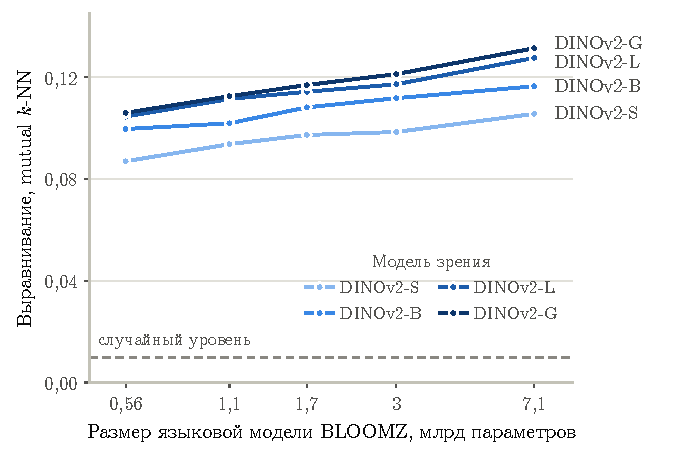
\includegraphics[width=0.75\textwidth]{figures/wit1024_alignment_article.pdf}
\caption{Выравнивание моделей BLOOMZ и~DINOv2 на наборе \mbox{WIT-1024} в~зависимости
  от размера языковой модели (логарифмическая шкала); пунктир~--- случайный
  уровень $k/(n-1)$}
\label{fig:exp0}
\end{figure}

Полученные значения согласуются с~опубликованными. В~\cite{koepke2026cave} на том~же
наборе при $k=10$ для пары \mbox{OpenLLaMA-3B} и~\mbox{DINOv2-base} получено 0,135. Воспроизводится
и~основной качественный вывод~\cite{huh2024platonic}: чем крупнее модели, тем сильнее
выровнены их представления. В~\cite{huh2024platonic} выравнивание сопоставляется также
с~качеством языковой модели, которое измеряется величиной $1-\mathrm{bpb}$ на тех~же
подписях, где bpb~--- число бит на байт текста~\cite{koepke2026cave}. В~проведённом
эксперименте значение bpb, рассчитанное по коду авторов, составило от 1,84 до 2,03
и~не убывало монотонно с~размером модели: у~\mbox{BLOOMZ-1b7} оно выше, чем у~\mbox{BLOOMZ-1b1}.
По-видимому, на коротких подписях и~для моделей, дообученных на наборе задач
с~текстовыми инструкциями~\cite{muennighoff2023bloomz}, эта величина плохо отражает
качество модели, поэтому на рис.~\ref{fig:exp0} выравнивание показано в~зависимости
от числа параметров.

Эксперимент показывает, что реализация меры и~процедура извлечения представлений
воспроизводят результат~\cite{huh2024platonic}, но не снимает возражений против самого
результата. Выборка из 1024 пар с~однозначным соответствием мала:
в~\cite{koepke2026cave} при расширении галереи до 15~млн пар из набора LAION значение
для той~же пары моделей падает с~0,135 до 0,008. Контрольное значение на перемешанных
парах вычислялось для уже выбранной пары слоёв, тогда как выбор максимума по всем парам
слоёв сам по себе немного завышает оценку. Наконец, использовались одна подпись
на изображение и~одно значение~$k$. Эти ограничения учитываются в~основной части работы:
калибровка будет выполняться с~тем~же выбором слоёв, что и~для исходных пар, а~мера
будет вычисляться на выборках разного размера и~при нескольких значениях~$k$.

%======================================================================
\section{План основных экспериментов}\label{sec:plan}

Следующий этап~--- применение протокола к~рекомендательным моделям. Первый эксперимент
проводится на наборе \mbox{MovieLens-1M}~\cite{harper2015movielens}, который содержит около
миллиона оценок 6040 пользователей примерно для 3,7~тыс. фильмов. Оценки
рассматриваются как факты взаимодействия и~упорядочиваются по времени, а~описанием
фильма служат его название, год выпуска и~жанры. Строки матриц~$F$ и~$G$ сопоставляются
по идентификатору фильма, что задаёт однозначное соответствие между представлениями.

Рекомендательные модели~--- матричное разложение, Item2Vec~\cite{barkan2016item2vec}
и~SASRec~\cite{kang2018sasrec}~--- обучаются с~нуля при нескольких размерах
представлений и~долях обучающих данных; представления фильмов берутся из их матриц
векторных представлений товаров. Описания фильмов кодируются языковыми моделями
нескольких размеров тем~же способом, что и~подписи в~разделе~\ref{sec:exp0}. Для каждой
пары моделей вычисляются калиброванные меры~\eqref{eq:calib}, а~для каждой
рекомендательной модели~--- Recall@$K$, NDCG@$K$ и~сходство с~эталоном~\eqref{eq:pmi}.
Ориентиром служит сходство моделей одной архитектуры, различающихся только начальной
инициализацией: оно показывает, насколько близки представления, полученные из одних
и~тех~же данных. Чтобы проверить устойчивость выводов к~размеру выборки, меры
вычисляются также на подмножествах фильмов разного размера с~числом соседей~$k$,
согласованным с~размером выборки~\cite{koepke2026cave}.

%======================================================================
\section{Заключение}

В~работе сформулирована постановка задачи проверки сходимости представлений
рекомендательных моделей: заданы внутренний и~внешний критерии, калиброванная мера
сходства и~эталон на основе совместной встречаемости товаров. Реализация меры
проверена на воспроизведении эксперимента~\cite{huh2024platonic}. На наборе \mbox{WIT-1024}
выравнивание языковых моделей BLOOMZ и~моделей зрения DINOv2 в~9--13 раз превышает
случайный уровень и~растёт с~размером обеих моделей, а~его величина согласуется
с~опубликованной в~\cite{koepke2026cave}. Малый размер выборки ограничивает силу этого
вывода, поэтому в~экспериментах на MovieLens сходство будет измеряться с~калибровкой
и~на выборках разного размера.

%======================================================================
\FloatBarrier
\begin{otherlanguage*}{english}
\bibliographystyle{IEEEtran}
\bibliography{refs}
\end{otherlanguage*}

\end{document}
